\section{Dynamische Geschäftsprozesse auf Basis von Ereignisverarbeitung}\label{sec:Kombi}
Bei der Automatisierung von Geschäftsprozessen und deren dynamischen Eigenschaften wächst, der Bedarf auf kritische Ereignisse in Echtzeit und ohne Latenzen zu reagieren.
Um den steigenden Anforderungen nach Echtzeitmanagement von Geschäftsprozessen unter Betrachtung relevanter Ereignisse zur Laufzeit gerecht zu werden, stellt die Integration von Ereignisverarbeitungskonzepten in die serviceorientierte Geschäftsprozessautomatisierung ein geeignetes Mittel dar. Die Vorteile für ein Unternehmen bei einer solchen Vervollständigung von Geschäftsprozessautomatisierung mit Konzepten der Ereignisverarbeitung sind im Wesentlichen durch folgenden Charakteristika fundiert:

\begin{itemize}
    \item 
    Identifikation relevanter oder kritischer Situationen für den Geschäftsprozess durch Berücksichtigung externer Ereignisse aus dem Geschäftsumfeld und interner Ereignisse aus dem Geschäftsprozess
    \item 
    Möglichkeit der unmittelbaren Reaktion auf veränderliche Situationen durch Verarbeitung von Ereignissen in Echtzeit
    \item
    Automatisierte Adaptionen von Geschäftsprozessen auf Basis von aktuellen Ereignissen
    \item
    Möglichkeit der Separierung der Ereignisverarbeitungslogik von der Geschäftsprozesslogik aufgrund von loser Kopplung und Kommunikation mittels Ereignisobjekten
    \item
    Gute Unterstützung verteilter Umgebungen, die insbesondere in unternehmensübergreifenden Geschäftsprozessnetzwerken und \ac{SOA}-Umgebungen eine bedeutende Rolle spielen
\end{itemize}

Es existieren bereits erste Forschungsansätze mit dem Ziel der Anreicherung von Geschäftsprozessmodellen mit Konzepten der Ereignisverarbeitung, die unter der englischen Bezeichnung Event- Driven Business Process Management (EDBPM) subsumiert werden. Publikationen aus diesem Bereich werden in den folgenden Abschnitten vorgestellt und anschließend anhand wesentlicher Kriterien gegenübergestellt.
\todo{Überarbeiten}

\subsection{Merkmale und Kriterien}

Dynamische und somit ereignisorientierte Geschäftsprozesse operieren prinzipiell auf zwei Ebenen, der Geschäftsprozessebene und der Ereignisverarbeitungsebene. 
Diese erfüllen ihre Aufgaben in erster Linie separat und in paralleler Weise, kommunizieren allerdings mittels des Austauschs von Ereignissen miteinander, was in diesem Kontext den maßgeblichen Aspekt darstellt. Abbildung \ref{fig:Ebenen dynamischer Geschäftsprozesse} illustriert in schematischer Darstellung die Zusammenhänge.

Auf der Ereignisverarbeitungsebene werden eingehende Ereignisse aus diversen externen und internen Ereignisquellen kontinuierlich analysiert, wobei zudem Ereignisse generiert werden können, welche wiederum dieselbe Analyse durchlaufen. 
Da zwischen der Ereignisverarbeitungsebene und der Geschäftsprozessebene mit Ereignissen kommuniziert werden kann, können diese generierten Ereignisse als unmittelbare Reaktion eine dynamische Wirkung auf den Ablauf des laufenden Geschäftsprozess ausüben.
Der Geschäftsprozess fungiert demnach einerseits als eine der internen Ereignisquellen für die Ereignisverarbeitungsebene und andererseits als wesentlicher Ereigniskonsument der generierten Ereignisse zur Adaption des Prozessablaufs.

\begin{figure}[H]
	\centering 
    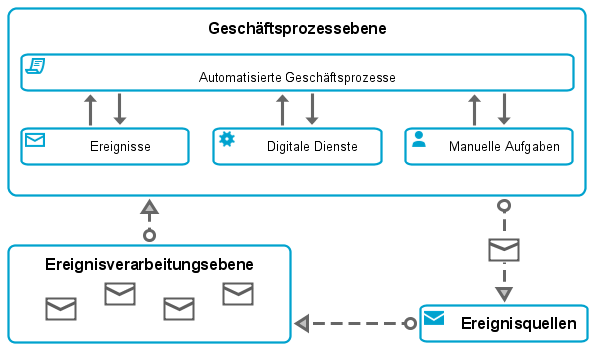
\includegraphics[width=\textwidth]{img/dynamicbp.png}	
    \caption[Ebenen dynamischer Geschäftsprozesse]
    {Ebenen dynamischer Geschäftsprozesse \protect\footnotemark}
    \label{fig:Ebenen dynamischer Geschäftsprozesse}
\end{figure}
\footnotetext{in Anlehnung an \citeauthor{Vidackovic.2014} \citeyear{Vidackovic.2014} \cite{Vidackovic.2014} }

Auf der Geschäftsprozessebene erfolgt der operative und automatisierte Ablauf von Aktivitäten des Geschäftsprozesses, wobei Letztere in einer \ac{SOA} überwiegend auf elektronischen Diensten basieren, die als Webservices über standardisierte Schnittstellen aufgerufen werden und auch über Unternehmensgrenzen hinweg verteilt sein können.
Bei den Aktivitäten kann es sich darüber hinaus auch um manuelle Benutzeraufgaben handeln, die zwar von Menschen ausgeführt werden, aber dennoch mittels informationstechnischen Schnittstellen in einen automatisierten Prozessablauf integriert werden können.

In ereignisorientierten im Gegensatz zu ablauforientierten Geschäftsprozessen üben Ereignisse zur Laufzeit einen signifikanten Einfluss auf den Prozessablauf aus, sodass die Geschäftsprozesse anhand geeigneter Ereignisverarbeitungsregeln mit dynamischen Eigenschaften ausgestattet werden können. 

\todo{Überarbeiten und Quellen}

\subsection{Gegenüberstellung vorhandener Forschungsansätze}
Die wesentlichen Aspekte der existierenden Forschungsansätze werden zunächst einzeln betrachtet und anschließend gegenübergestellt.

\todo{Forschungsansätze ausformulieren}

\paragraph{Entwicklung agiler Geschäftsprozesse mit Ereignisverarbeitung}
Dieser Forschungsansatz liefert eine Methode und Modelle zur Entwicklung agiler und zur Laufzeit anpassbarer Geschäftsprozesse, die nicht als Gesamtheit modelliert werden, sondern lediglich aus einzelnen Ereignis-Aktivität-Einheiten bestehen. Diese werden zur Laufzeit mithilfe von Ereignisverarbeitung ausgeführt und fügen den Geschäftsprozess dynamisch zusammen, wobei neue Ereignis-Aktivität-Einheiten agil hinzugefügt werden können. Die fachliche Modellierung von Ereignisverarbeitungsregeln beinhaltet kausale, logische und temporäre Beziehungen zwischen Ereignissen. Auch wird eine konzeptionelle Architektur für eine Ausführungsumgebung vorgeschlagen. 

Ein Defizit dieses Forschungsansatzes ist die fehlende Behandlung der Ausführungssemantik und die Missachtung wesentlicher Konzepte der Ereignisverarbeitung, wie beispielsweise verschiedener Fenster und Operatoren. Das interessante Konzept der Ereignis-Aktivität-Einheiten wird auch in dieser Arbeit aufgegriffen, allerdings ausgehend von einem in seiner Gesamtheit modellierten Geschäftsprozess, der in diese Einheiten zerlegt wird.
\cite{Alexopoulou.2008}
\todo{Überarbeiten}

\paragraph{RESTful SOA zur Automatisierung von Geschäftsprozessen}
Die Realisierung von SOA erfolgt in diesem Beitrag konform zum Architekturstil REpresentational State Transfer (REST).
Durch den Entwurf serviceorientierter Architekturen nach den Bedingungen und Technologien von REST entsteht die RESTful SOA. Zielsetzung des vorliegenden Beitrags ist die modellbasierte Spezifikation von RESTful SOA zur Automatisierung von Geschäftsprozessen. 

In aktuellen Praxis- und Forschungsarbeiten zu diesem Thema liegt der Fokus jedoch auf der softwaretechnischen Spezifikation von RESTful SOA. Dagegen findet eine durchgängige Entwicklung ausgehend von den Anforderungen in modellierten Geschäftsprozessen nur wenig Beachtung.
Die Konstruktion eines modellbasierten Entwicklungsvorgehens zur Spezifikation von RESTful SOA ausgehend von Geschäftsprozessmodellen bildet die Problemstellung dieser Arbeit.

Hierbei sind insbesondere das Überwinden der semantischen Lücke zwischen Geschäftsprozessmodell und Anwendungssystem durch ein systematisches Vorgehen sowie das Sicherstellen einer konsistenten Abstimmung von AwS mit den Geschäftsprozessmodel- len von hoher Bedeutung. Die aufgezeigten Probleme werden durch einen Ansatz zur modellbasierten, metho- disch geleiteten Ableitung der softwaretechnischen SOA-Spezifikation auf Basis von Geschäftsprozessmodellen angegangen.

Das vorgestellte methodisch gestützte Vorgehen leitet den Entwickler bei der schritt- weisen Überbrückung der semantischen Lücke zwischen fachlichem Geschäftsprozess und softwaretechnischer AwS-Spezifikation an. Zur Bewältigung der Komplexität tragen zudem die Trennung von struktur- und verhaltensorientierter Sicht auf den verschiedenen Modellebenen der SOM-Methodik und ihre durchgängige Modellierung bei. Die Anwendbarkeit des Ansatzes und das Ziel der Erhöhung der Konsistenz zwischen Implementierung und Dokumentation des Informationssystems wurden anhand der Fallstudie aufgezeigt und die Ergebnisse reflektiert. Der Einsatz des eingeführten modellbasierten Vorgehens ermöglicht zudem die Verbesserung von Zeit-, Kosten- und Qualitätsmerkma- len des Systementwicklungsprozesses.
\cite{Wolf.2016}
\todo{Überarbeiten}

\paragraph{SOEDA-Methode}
SOEDA bezeichnet eine Methode zur Entwicklung von Anwendungen durch die Verschmelzung aus dienstorientierten (SOA) und ereignisgesteuerten Architekturen (EDA). Geschäftsprozesse werden hier mit EPK modelliert und in WS-BPEL transformiert. Mithilfe einer rudimentären Technik zur Ereignisverknüpfung werden die komplexen Ereignisse aus dem Geschäftsprozessmodell mittels grafischer und nicht-formaler Modellierung auf die zugrunde liegenden singulären Ereignisse heruntergebrochen, sodass anschließend ein Entwickler die Ereignisverarbeitungsregeln von Hand in einer Engine-spezifischen Ereignisverarbeitungssprache implementieren kann. Durch Hinzufügen technischer Details zum WS-BPEL-Modell wird das Geschäftsprozessmodell schließlich ausführbar.

Schwächen der SOEDA-Methode liegen in der unzulänglichen Modellierung von Ereignisverarbeitungsregeln und dem Fehlen einer automatischen Transformation in ein ausführbares Ereignis- verarbeitungsmodell. Auch mangelt es an dynamischen Anpassungen des Geschäftsprozesses zur Laufzeit, da Ereignisse lediglich als Bestandteil des regulären Geschäftsprozessablaufs betrachtet werden. Ab Version 2.0 verfügt die BPMN neben einer grafischen Notation nun auch über die technische Ausführungssemantik und ist somit direkt in einer Engine ausführbar. Somit erscheint der Umweg einer Transformation von EPK zu WS-PEL als nicht mehr erforderlich, zumal eine Konsistenz im Geschäftsprozessmodell auf Geschäfts- und technischer Ebene erstrebenswert ist
\cite{MatthiasWieland.2009} 
\cite{Bruns.2010}S.37
\cite{RobraBissantz.2009}
% SOEDA bezeichnet eine Methode zur Entwicklung von Anwendungen durch die Verschmelzung aus dienstorientierten (SOA) und ereignisgesteuerten Architekturen (EDA). Geschäftsprozesse werden hier mit EPK modelliert und in WS-BPEL transformiert. Mithilfe einer rudimentären Technik zur Ereignisverknüpfung werden die komplexen Ereignisse aus dem Geschäftsprozessmodell mittels grafischer und nicht-formaler Modellierung auf die zugrunde liegenden singulären Ereignisse her- untergebrochen, sodass anschließend ein Entwickler die Ereignisverarbeitungsregeln von Hand in einer Engine-spezifischen Ereignisverarbeitungssprache implementieren kann. Durch Hinzufügen technischer Details zum WS-BPEL-Modell wird das Geschäftsprozessmodell schließlich ausführbar.

% Schwächen der SOEDA-Methode liegen in der unzulänglichen Modellierung von Ereignisverarbeitungsregeln und dem Fehlen einer automatischen Transformation in ein ausführbares Ereignis- verarbeitungsmodell. Auch mangelt es an dynamischen Anpassungen des Geschäftsprozesses zur Laufzeit, da Ereignisse lediglich als Bestandteil des regulären Geschäftsprozessablaufs betrachtet werden. Ab Version 2.0 verfügt die BPMN neben einer grafischen Notation nun auch über die tech- nische Ausführungssemantik und ist somit direkt in einer Engine ausführbar. Somit erscheint der Umweg einer Transformation von EPK zu WS-BPEL als nicht mehr erforderlich, zumal eine Konsistenz im Geschäftsprozessmodell auf Geschäfts- und technischer Ebene erstrebenswert ist.



\paragraph{Gegenüberstellung der Ansätze}